\documentclass{life-fr}

\begin{document}

\title{La Vie est un Jeu}
\subtitle{Bilan Architecture}
\member{Lepage Barbara}{lepage.barbara@gmail.com}
\member{Caradec Guillaume}{guillaume.caradec@gmail.com }
\member{Corsin Simon}{simoncorsin@gmail.com }
\member{Glorieux François}{fra.glorieux@gmail.com}
\member{Klarman Nicolas}{nickoas@gmail.com}
\member{Lassagne David}{david.lassagne@gmail.com}
\member{Louvigny Guillaume}{guillaume@louvigny.fr}
\member{El-Outmani Youssef}{youssef.eloutmani@gmail.com}
\member{Le-Cor Wilfried}{wilfried.lecor@gmail.com}
\member{Lenormand Frank}{lenormf@gmail.com}

\summary
{
  Ce bilan a pour but de vérifier la bonne conception de l’architecture
  du projet.
}

\maketitle
\authorspage

%% --------------------------------------------------------------------- %%

\chapter*{Résumé}
{
  «~La Vie Est Un Jeu~» est un projet sur trois ans dans le cadre des «~Epitech
  Innovative Projects~» mené par un groupe de dix étudiants.\\
  \\
  Ce projet, sous forme d'un site web et d'applications mobiles, propose à
  ses utilisateurs de pimenter leur quotidien. Pour cela, on leur propose
  de manière ludique de se fixer des objectifs, les réaliser, les collectionner
  et enfin les partager.\\
  C'est donc à la fois un jeu et un réseau social, destiné à tous les âges !\\
  \\
  TODO
}

\chapter*{Informations du document}

\begin{tabular}{ | m{5cm} | m{10cm} | }
  \hline
  Type du document & Bilan Architecture\\
  \hline
  Nom du groupe & La Vie Est Un Jeu\\
  \hline
  Nombre de pages & \ref{TotPages} \\
  \hline
  Titre complet du document & Bilan Architecture du projet «~La Vie Est Un Jeu~»\\
  \hline
  Auteurs & Membres du groupe, voir page de garde\\
  \hline
  Responsable & Chef de groupe : Barbara Lepage\\
  \hline
  Contact & lavieestunjeu@googlegroups.com\\
  \hline
  Mots clés & «~bilan~», «~architecture~», «~UML~», «~diagrammes~», «~conception~», «~bases de données~», «~lavieestunjeu~»\\
  \hline
  Révision actuelle & 1.0\\
  \hline
  Site vitrine & http://eip.epitech.eu/2014/lavieestunjeu/\\
  \hline
  Site officiel & Non disponible\\
  \hline
\end{tabular}

\chapter*{Table des révisions}

\revision{0.1}{Lepage Barbara}{Rappel de l'EIP}{11/07/2012}
\listofrevisions

\newpage

\tableofcontents

%% --------------------------------------------------------------------- %%

\chapter{Introduction et contexte}

\section{Epitech, l'EIP et «~La Vie Est Un Jeu~»}

\subsection{Epitech, une école d'informatique pas comme les autres}

Epitech est une école formant des experts en informatique. Sa pédagogie par projets
implique directement les étudiants dans leur apprentissage et les rend plus à même
de réagir et s'adapter aisément, par exemple aux évolutions technologiques qui
auront lieu au cours de leur carrière.

\subsection{L'EIP, élément clé de la réussite scolaire}

Un Epitech Innovative Project ou EIP est l'élément clé du cursus Epitech. Il s'agit d'un projet de fin d'études regroupant un minimum de six étudiants autour d'un but commun. Ce projet est conduit sur une durée de trois ans, beaucoup plus importante que celles des projets réalisés lors des trois premières années d'études. De plus, l'EIP amène les étudiants à se confronter au monde de l'entreprise.

\subsection{«~La vie est un Jeu~», bien plus qu'un simple EIP : une révolution !}

Dans le cadre de notre EIP, nous avons décidé de réaliser un réseau social à but ludique basé sur les «~listes de choses à faire avant de mourir~» : il définit toutes les choses que son auteur désire faire de son existence, une sorte de mémo pour ne pas gâcher sa vie. Notre projet permettra à nos visiteurs de construire leurs propres listes et de faire valider leurs exploits tout en les partageant avec leurs réseaux sociaux. Ainsi, chaque action réalisée par un utilisateur (ajout d'une activité, succès ou échec) sera un fil de discussion dans lequel le visiteur et son réseau pourront discuter et partager différents types de médias (photos, vidéos, etc.). Ce fil de discussion se trouvera sur les flux d'informations propres à chacun. L'activité d'un utilisateur sera validée par son propre réseau et apparaîtra sous forme de «~succès~», comme dans un jeu vidéo. Le site s'étendra par la suite en proposant d'autres caractéristiques propres aux jeux vidéo.

%% --------------------------------------------------------------------- %%

\section{Vocabulaire du projet}

\subsection{Qu'est-ce qu'un «~achievement~» ?}
Le terme achievement (qui peut être traduit par succès ou réalisation en français) est, dans le cadre vidéoludique,  un objectif défini à accomplir par le joueur, en dehors de l’objectif principal (c’est-à-dire, gagner ou finir le jeu).\\
 Les achievements sont donc des récompenses honorifiques ajoutant du challenge pour le joueur.\\
\\
Nous pourrions utiliser une traduction française du terme achievement mais nous pensons que achievement est le terme le plus populaire dans le monde vidéoludique.\\
\\
Les achievements permettent au joueur de découvrir plus en profondeur le contenu du jeu et donc d’explorer de nouveaux horizons.\\
 L’obtention est souvent un moment agréable pour le joueur.\\
 Il ressent une certaine satisfaction et se sent récompensé pour un effort.\\
 Il peut ensuite les partager avec ses amis afin de recueillir les honneurs ou défier ses amis de faire autant ou mieux, ce qui améliore grandement l’immersion au sein du jeu.\\
\\
Nous pensons, qu’il est intéressant d’en faire une analogie avec la vie.\\
 La vie est un jeu comme un autre et mérite d’avoir elle aussi ses achievements.

\subsection{Définitions, Acronymes et Abréviations}

\begin{description}
\item[Algorithme]
Suite finie et non-ambiguë d’instructions permettant de donner la réponse à un problème.
\item[API]
En français «~Interface de Programmation~», c'est une interface fournie par un programme informatique permettant l'interaction des programmes les uns avec les autres.

\item[Application mobile]
Une application mobile est une application développée pour être installée sur un appareil électronique mobile.

\item[Architecture web]
Une architecture web désigne la structure générale inhérente à un environnement web.

\item[Base de données]
Une base de données est un lot d'informations stockées dans un dispositif informatique.

\item[Breaking news]
En français «~Dernières Nouvelles~».

\item[Bug tracker]
En français «~Logiciel de suivi de problèmes~», c'est un logiciel permettant d'aider les utilisateurs et les développeurs à améliorer la qualité d'un logiciel en trouvant les failles de celui-ci.

\item[Cahier des charges]
Le Cahier des charges vise à définir simplement les spécifications d’un produit ou d’un service à réaliser.

\item[Dépôt]
Un dépôt est un stockage centralisé et organisé de données.

\item[Diagramme de Gantt]
Un diagramme de Gantt est un outil utilisé en ordonnancement et gestion de projet et permettant de visualiser dans le temps les diverses tâches liées composant un projet.

\item[Diaporama]
Un diaporama est une suite d’images ou de documents reliés par des effets et sur lesquels il est possible de mettre du son.

\item[Doodle]
Doodle.com est un site web de planification et de sondage de la société suisse Doodle AG.

\item[GitHub]
Github est un service web d'hébergement et de gestion de développement de logiciels, utilisant le programme Git.

\item[Google Docs]
Google Docs est la suite des évolutions de Google Spreadsheets, logiciel de traitement de texte. Ces programmes fusionnés permettent un travail collaboratif en ligne.

\item[Google Talk]
Google Talk est un logiciel propriétaire et service de messagerie instantanée et de voix sur IP basé sur Jabber et développé par la société Google.

\item[IRC]
IRC est un protocole de communication textuelle sur Internet.

\item[JavaScript]
JavaScript est un langage de programmation de scripts principalement utilisé pour les pages web interactives.

\item[Login]
En français «~Identifiant~», c'est une information permettant à une personne de s'identifier auprès d'un système.

\item[Mailing list]
En français «~Liste de diffusion~», c'est une utilisation spécifique du courrier électronique qui permet le publipostage d'informations aux utilisateurs qui y sont inscrits.

\item[Mise en production]
Mise à disposition totale d’un service ou d’un produit.

\item[Ocaml]
Anciennement connu sous le nom d'Objective Caml, c’est l'implémentation la plus avancée du langage de programmation Caml.

\item[Ocsigen]
Framework de développement web, développé par le laboratoire français PPS.

\item[Réseau]
Maillage de liens entre différents équipements informatiques permettant un partage d’informations.

\item[Réseau social]
Ensemble d'identités sociales, telles que des individus ou encore des organisations, reliées entre elles par des liens créés lors d’interactions sociales.

\item[Service]
Apporte une valeur ajoutée à un produit ou assure un travail nécessaire à une entreprise ou à un particulier.

\item[Site vitrine]
Site internet composé de quelques pages présentant une société. Permet à une entreprise de communiquer avec le monde.

\item[Smartphone]
Téléphone mobile disposant aussi des fonctions d'un assistant numérique personnel. Il fournit des fonctionnalités basiques comme l'agenda, le calendrier, la navigation sur le Web, la consultation du courrier électronique, la messagerie instantanée, le GPS, ...

\item[Android]
Système d’exploitation utilisant le noyau Linux pour smartphones, PDA et terminaux mobiles conçu par Android, une startup rachetée par Google.

\item[iOS]
Système d’exploitation mobile développé par Apple pour l'iPhone, l'iPod touch, et l'iPad. Il est dérivé de Mac OS X dont il partage les fondations.

\item[Windows Phone]
Système d’exploitation mobile développé par Microsoft pour succéder à Windows Mobile, sa précédente plate-forme logicielle.

\item[Version Bêta]
Version de test comportant toutes les fonctionnalités d'un programme. C'est grâce à cette version que les testeurs remontent les éventuels problèmes.

\item[Wiki]
Espace collaboratif sur lequel les utilisateurs sont invités à rédiger des documents de travail.


\end{description}


%% --------------------------------------------------------------------- %%

\section{Pré-requis et informations sur le projet}

\subsection{Destinataires du projet}

Les utilisateurs ciblés par le projet sont très nombreux. Il suffit qu'une personne ait un centre d'intérêt ou une passion couvert(e) par le site pour qu'elle ait une raison de s'y inscrire.\\

Le site comme les applications mobiles seront conçus en vue d'une internationalisation étendue.

\subsection{Utilisation du projet, rapport à l'existant}

Pour les utilisateurs finaux, le projet sera composé d'un site web et de plusieurs applications mobiles incluant Android, iOS et Windows Phone. Pour les développeurs tiers, une API sera mise en service, permettant la création de nouveaux usages.\\

Le projet a été pensé de façon à pouvoir répondre à un ensemble de fonctionnalités non présentes dans les projets déjà existants. Ces fonctionnalités ne sont pas combinées ou présentes sur les sites concurrents. En effet, nous tenons à mettre en place une plate-forme suffisamment ludique pour être visitée au quotidien, sans pour autant négliger l’aspect social permettant au visiteur de discuter de ses loisirs avec son réseau et de pouvoir partager aisément ses expériences à travers photos et vidéos.\\

À l'issue de la première année de travail sur le projet en partenariat avec l'INRIA et le Koalab Epitech, nous estimons avoir un site fonctionnel. Pendant la seconde année de travail sur l'EIP nous aimerions pouvoir signer des partenariats commerciaux avec divers acteurs de domaines culturels ou encore événementiels. Cette période sera également l'occasion d'ajouter de nouvelles fonctionnalités annexes répondant à des besoins émanant par exemple des utilisateurs.

\newpage

\subsection{Remise en contexte technologique}

Aujourd'hui, une part de plus en plus importante d'utilisateurs d'Internet sont équipés de smartphones, il est même prévu que le nombre d'utilisateurs en mobilité dépasse celui des utilisateurs sédentaires d'ici quelques années.\\
\\
Pour s’adapter à cette évolution et faire face à l’expansion notable de nouvelles technologies, nous avons choisi de proposer à nos utilisateurs des versions dédiées aux plates-formes mobiles majeures.

\subsection{But final du projet}

Le projet a pour but de créer une communauté d'utilisateurs autour d'un système d'achievements, directement lié à la vie quotidienne, aux passions ou à la vie professionnelle.\\

Les utilisateurs ciblés sont très nombreux. En théorie, toute personne ayant un centre d'interêt ou une passion est une cible.\\

À plus long terme, des partenariats commerciaux permettront de cibler des marques et des lieux.\\

Le site sera multilingue, donc ouvert à l'internationalisation.

\section{Références}

Ce document présente l’architecture du projet « La Vie Est Un Jeu ». Pour mieux le comprendre, il est
fortement recommandé de prendre connaissance des documents suivants :

\begin{description}

  \item[Étude de l’existant]
    Ce document présente les projets existants ressemblant au notre. En étudiant ainsi le marché, nous nous assurons d’éviter les erreurs de nos concurrents et d’en faire la solution la meilleure.

  \item[Cahier des charges]
    Ce document présente dans les détails les fonctionnalités qui seront présentes dans notre projet, les plates-formes sur lesquelles il sera disponible, la portabilité serveur/client, les technologies utilisées, les raisons du choix de celles-ci, une introduction à la base de donnée et enfin l’organisation générale du projet avec planning et outils.
  \item[Diagramme de Gantt]
    Ce diagramme détaille les phases d’avancement du projet, les tâches à réaliser, la durée pour les réaliser, les dates de début et les dates limites de celle-ci et enfin les responsables de chacune d’entre elles.

\end{description}

Ces documents peuvent être téléchargés sur notre site vitrine :

\url{http://eip.epitech.eu/2014/lavieestunjeu/}

% --------------------------------------------------------------------- %%

\chapter{Représentation de l’architecture globale}
%%Vous présenterez dans cette partie l’approche du document, comment est faite l’actuelle architecture et les points de vue qui vont être présentés, et pour chaque point de vue, quels sont les éléments qui vont être présentés 

TODO

% --------------------------------------------------------------------- %%

\chapter{Architecture, buts et contraintes}
\section{Objectifs spécifiques ayant un impact sur l’architecture}
%% Vous présenterez dans cette section, les objectifs que vous avez pour votre projet qui ont un impact sur l’architecture 

Nos objectifs, qui incluent la création d'un service web et d'un ensemble d'applications mobiles, ont un certains nombres de contraintes. Celles-ci peuvent impacter l'architecture du projet : comme l'organisation même du développement, de la communication ou encore le code, et ce qu'elles soient inhérentes aux technologies retenues ou aux facteurs géographiques imposés par l'école.

\section{Contraintes fonctionnelles}
%% Vous présenterez ici les contraintes fonctionnelles qui ont un impact sur l’architecture (A vous de chercher ce qu’est une contrainte fonctionnelle) 

Plusieurs contraintes fonctionnelles, provenant directement de l'organisation même du projet sont à noter. Il s'agit principalement du départ à l'étranger de la moitié de l'équipe, qui sera alors répartie sur un ensemble très large de fuseaux horaires : États-Unis Pacifique à Chine. Des outils de communication adaptés sont d'ors et déjà mis en place tels qu'une liste de diffusion (indépendante de celle fournie par le Lab EIP pour des raisons de goûts personnels), un bug tracker (fourni par Github) ou encore un canal IRC sur les serveurs de l'école (\#eip-life). Ces ressources permettent de palier à l'absence potentielle de communication de vive voix entre les différentes composantes de l'équipe. Cependant des réunions ponctuelles planifiées à intervalles réguliers auront toujours lieu via visio conférence pour que chacun puisse faire part de sa progression dans les diverses tâches qui lui auront été assignées.\\
\\
Une autre contrainte fonctionnelle que nous avons identifié est quant à elle matérielle. Il s'agit de la disponibilité des divers équipements proposés par le Lab EIP. Nous auront en effet besoin de plusieurs smart-phones pour réaliser les versions mobiles de notre projet. Si, l'équipe présente à Paris pourra faire usage de ces appareils les membres étudiant dans les universités partenaires d'EPITECH ne pourront pas en profiter. Il faudra soit qu'ils passent par leurs équipements personnels (ne couvrant généralement qu'une infime partie des modèles de téléphone d'un système d'exploitation donné), ou alors les émulateurs (Android) ou simulateurs (iOS, Windows Phone) ne reproduisant pas de façon optimale les conditions réelles d'utilisation des applications.\\
\\
Notre projet étant un service web des serveurs seront nécessaire pendant toute la réalisation de celui-ci que ce soit les phases de formation, de développement ou encore de déploiement. Dans un premier temps seul un serveur de capacité réduite est nécessaire, puisque nous n'auront pas à faire face à un trafic important. Cependant par la suite il sera nécessaire d'acquérir des machines plus performantes dans le cadre du déploiement du projet. Cette phase devrait arriver assez tôt, approximativement vers l'automne 2013 si l'on se fit au calendrier convenu avec le Lab EIP.\\
\\
La dernière contrainte fonctionnelle que nous avons mis en lumière est notre incapacité actuelle à réaliser des tâches nécessitant des compétences plus larges que le simple développement : comme la conception d'interfaces utilisateurs ergonomiques, la réalisation d'une charte graphique propre au site etc. Pour répondre à ces besoins nous aurons le choix de nous former ou alors de faire appel à des personnes compétentes, extérieures à l'école.

\section{Contraintes non fonctionnelles}
%% Vous présenterez ici les contraintes non fonctionnelles qui ont un impact sur l’architecture (A vous de cherche ce qu’est une contrainte non fonctionnelle) 

Une certaine émulation aura lieu dans le domaine de notre projet : quelques acteurs ont des projets relatifs au nôtre et seront potentiellement amenés à empiéter sur notre offre. Il faudra alors être amené à réagir promptement et convenablement à ces concurrents, tout en veillant à ne pas laisser un seul acteur avoir une position hégémonique sur ce secteur.\\
\\
Ocsigen, le framework web en Ocaml conçu par les équipes de l'INRIA est puissant et performant. Cependant, le fonctionnement du langage, directement issu des principes de la programmation fonctionnelle énoncés par Church dans les années 1930, tranche beaucoup trop de la programmation impérative pour permettre une adaptation rapide et aisée à celui-ci. La formation au langage et, à plus forte mesure au framework, prendra alors une part importante dans la réalisation du projet. \\
\\
Ocsigen apporte quelques limitations, par exemple le choix de la base de données, qui sera obligatoirement une PostgreSQL.\\
\\
La technologie que nous employons, Ocsigen, permet une telle réactivité sur le client web, cependant les processus de validations d'applications sur iOS ou Windows Phone restent un frein à cette même réactivité. \\
\\
Toujours sur le plan des applications mobile, il ne faut pas perdre de vue que les mêmes fonctionnalités sont à coder quatre fois pour cibler toutes les plates-formes. En effet, il n'est pas rare que des entreprises comme Facebook ou Twitter proposent à plusieurs jours d'intervalle entre les divers systèmes mobiles des améliorations, ou alors que des fonctionnalités soient manquantes sur certains OS.

% --------------------------------------------------------------------- %%

\chapter{Vue globale du projet}
\section{Cas d'utilisation principaux}
%% Vous présenterez ici les scénarios / fonctionnalités par un diagramme UML de use case par exemple 

Le schéma suivant présente les principaux cas d'utilisation du projet. Les acteurs retenus sont les administrateurs, les modérateurs, les entreprises ainsi que les utilisateurs classiques.

\newpage

\begin{figure}[H]
  \begin{center}
    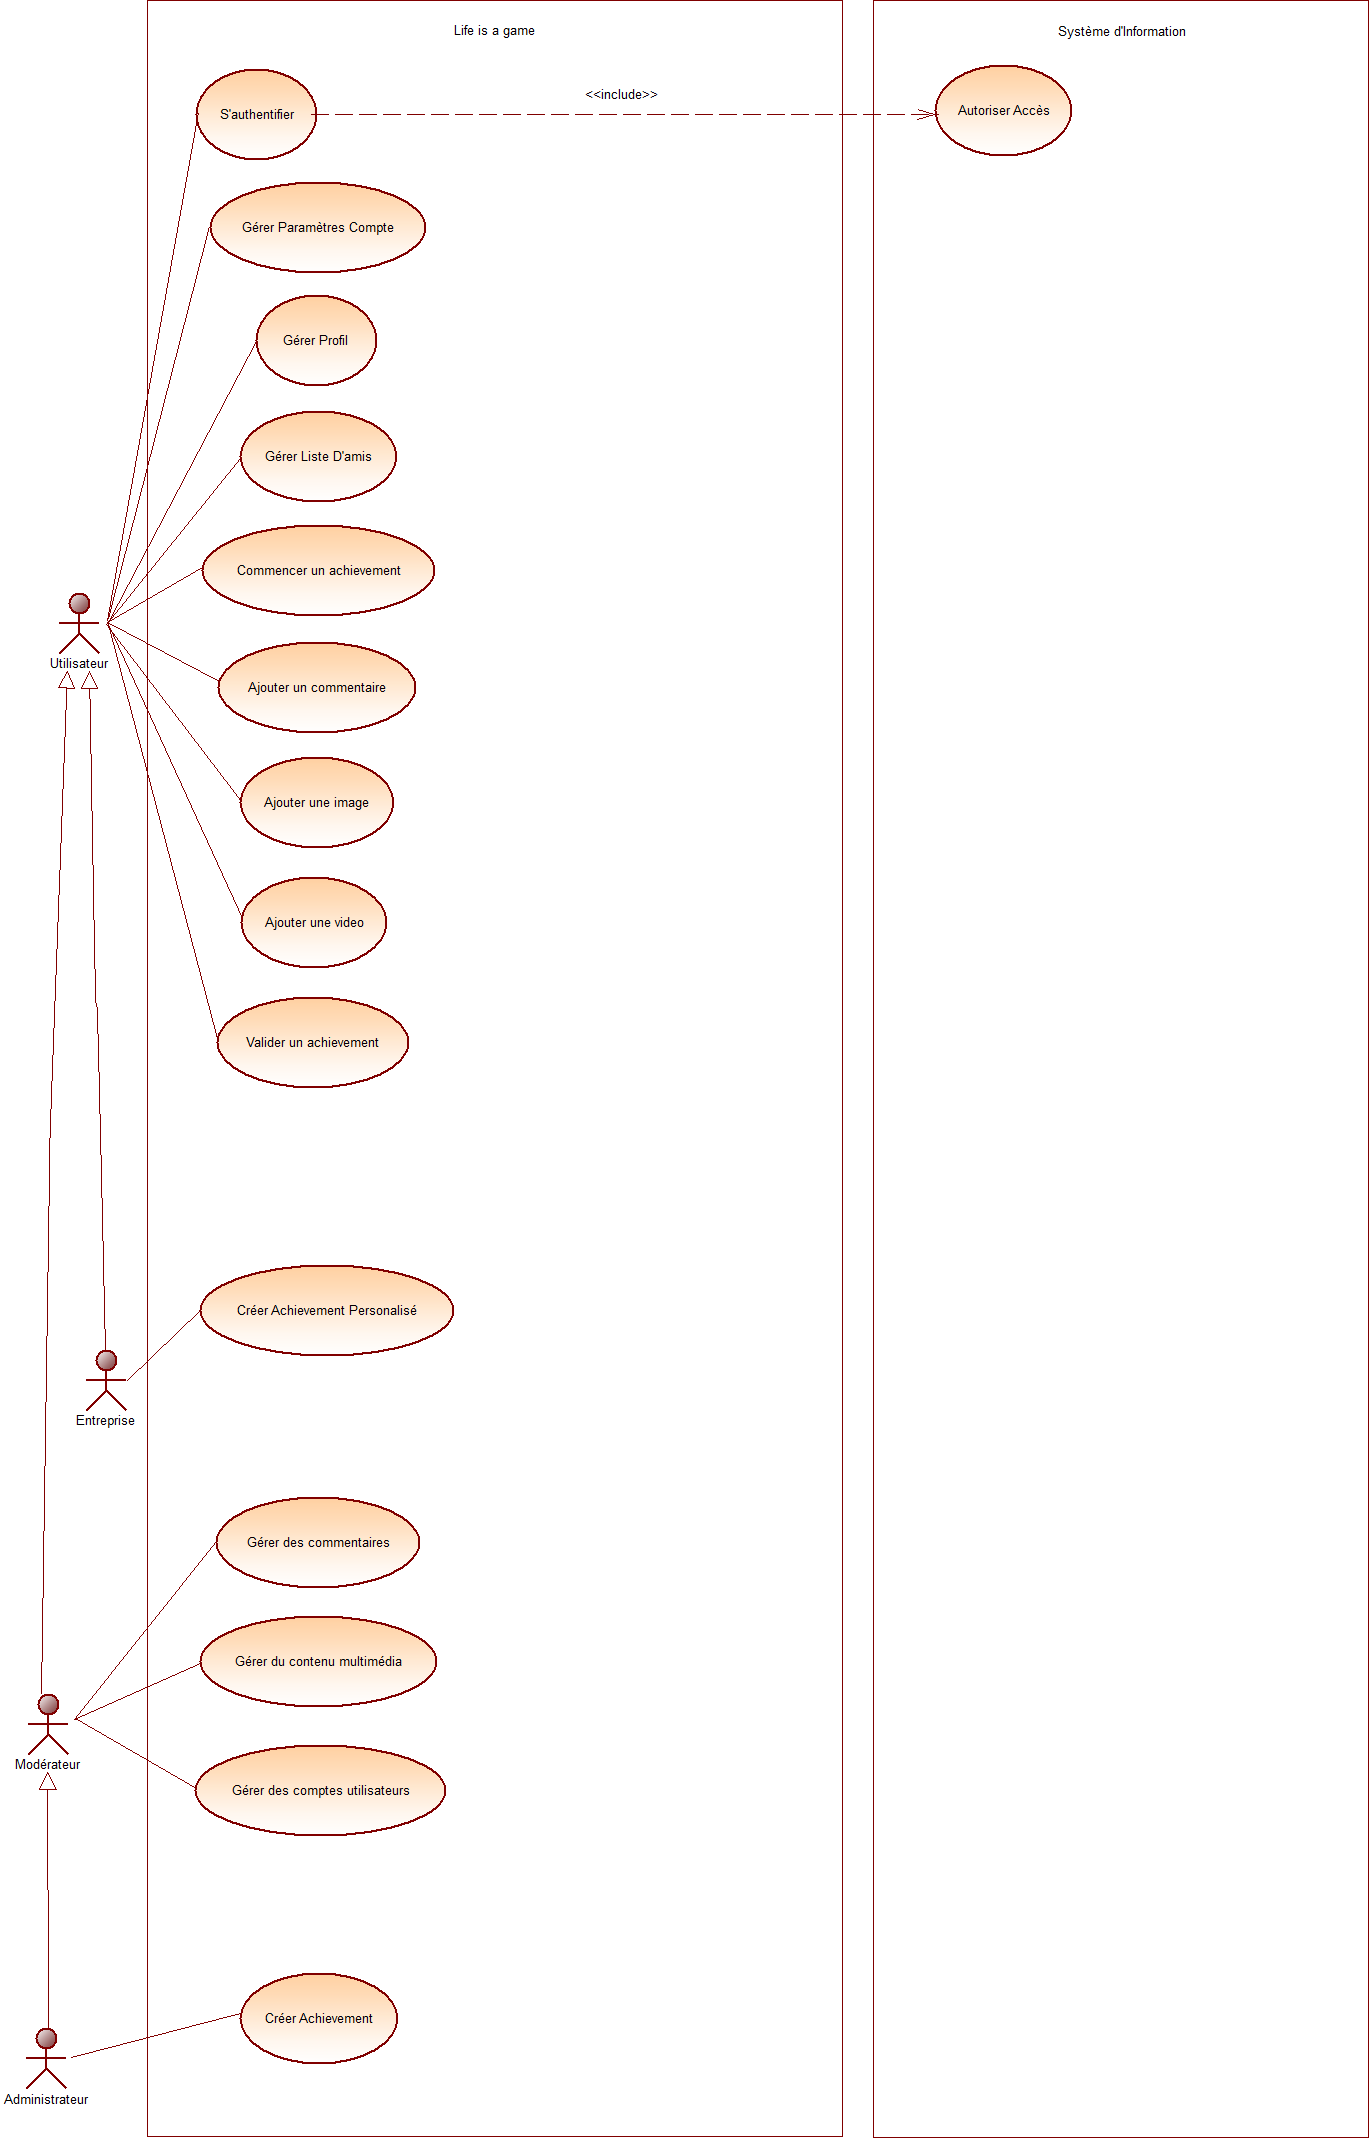
\includegraphics[width=15cm]{img/use_case_principaux.png}
  \end{center}
\end{figure}

\section{Cas d'utilisation détaillés}
%% Vous présenterez les UC détaillés dans ce paragraphe 

Le schéma qui suit expose les cas d'utilisation détaillés du projets, et ce pour un utilisateur dans le cadre de son inscription au service.

\begin{figure}[H]
  \begin{center}
    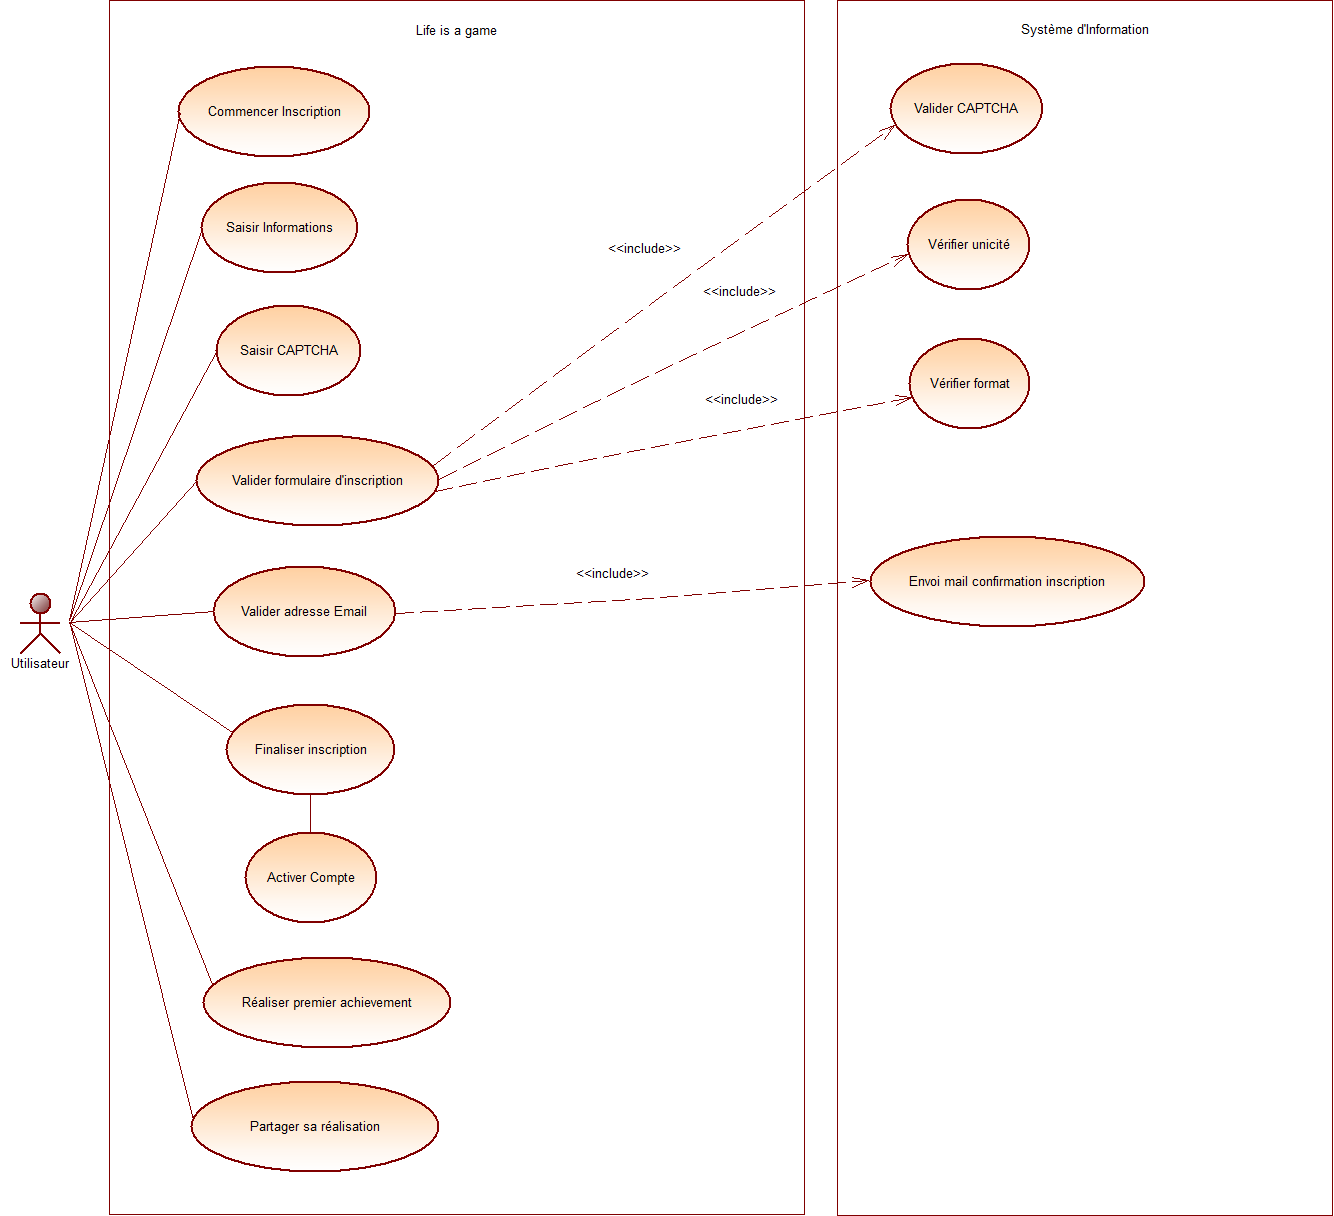
\includegraphics[width=17cm]{img/use_case_detailles.png}
  \end{center}
\end{figure}

% --------------------------------------------------------------------- %%

\chapter{Vue Logique de l’application}
\section{Vue globale}
%% Vous présenterez ici le design global de la solution, les composants, découpages en paquets, modules. Vous pourrez utiliser un diagramme de composants et/ou de déploiement UML 

TODO

\section{Composants principaux}
%% Vous décrirez ici les composants principaux utilisés, s’ils sont existants, créés, … 

TODO

% --------------------------------------------------------------------- %%

\chapter{Vue Processus}
%% Vous décrirez ici la décomposition en petites taches de votre système pour vous permettre de valider les processus et les acteurs mis en jeu dans les différentes fonctionnalités. Vous utiliserez par exemple des diagrammes de Séquence UML et Activité 

La série de schémas suivante expose diverses utilisations du projet, celle d'un utilisateur «~classique~» ayant un usage général de l'application, les fonctionnalités supplémentaires offertes à un modérateur, à une entreprise et aux modérateurs. Enfin l'inscription au service sera également détaillée.

\begin{figure}[H]
  \begin{center}
    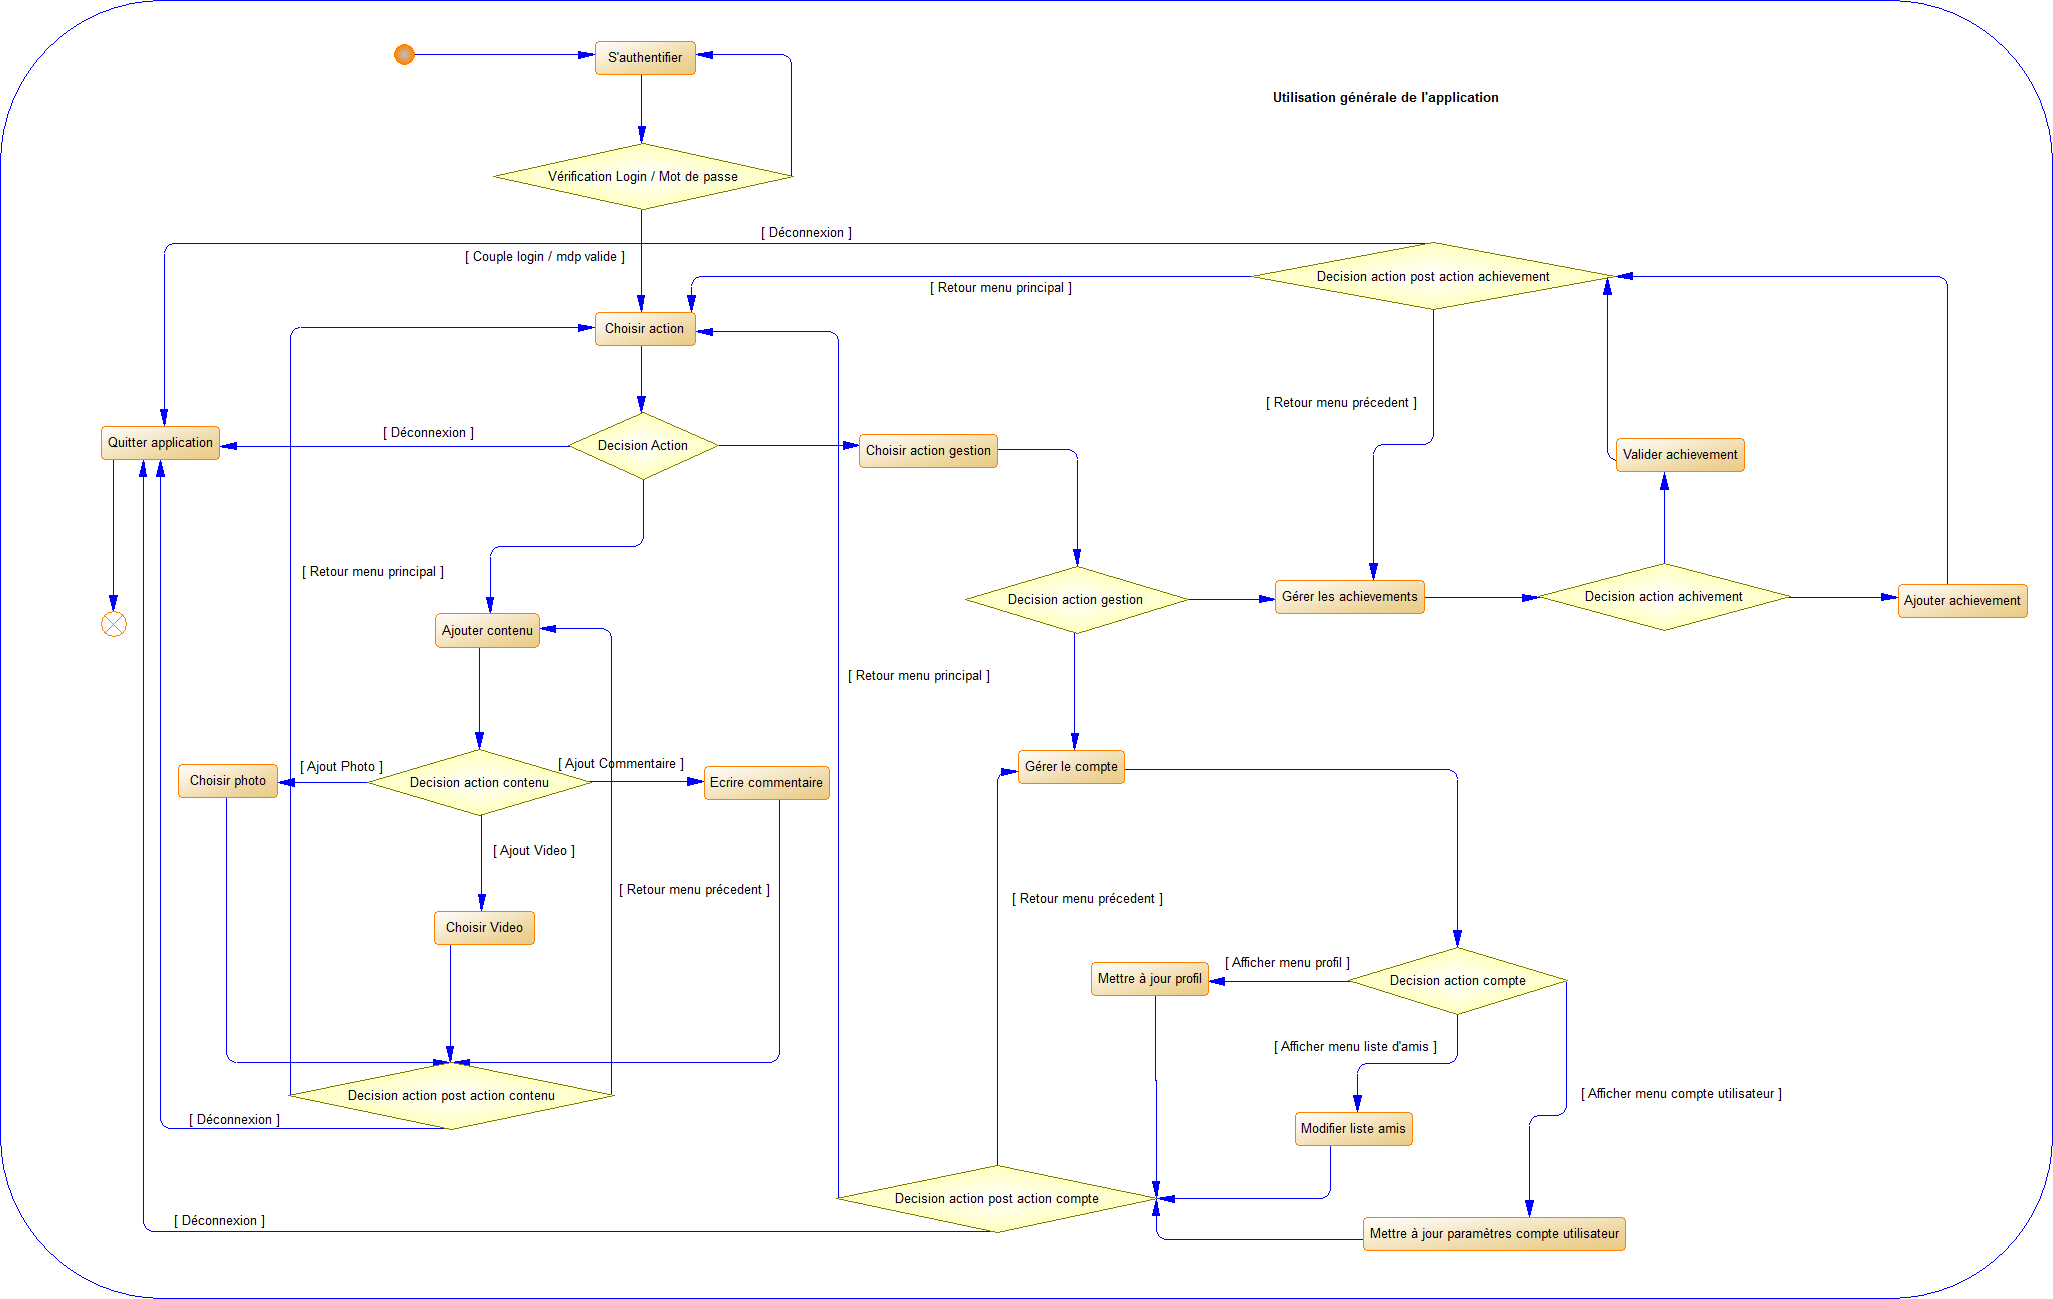
\includegraphics[width=17cm]{img/processus_principaux_2.png}
  \end{center}
\end{figure}

\newpage

\begin{figure}[H]
  \begin{center}
    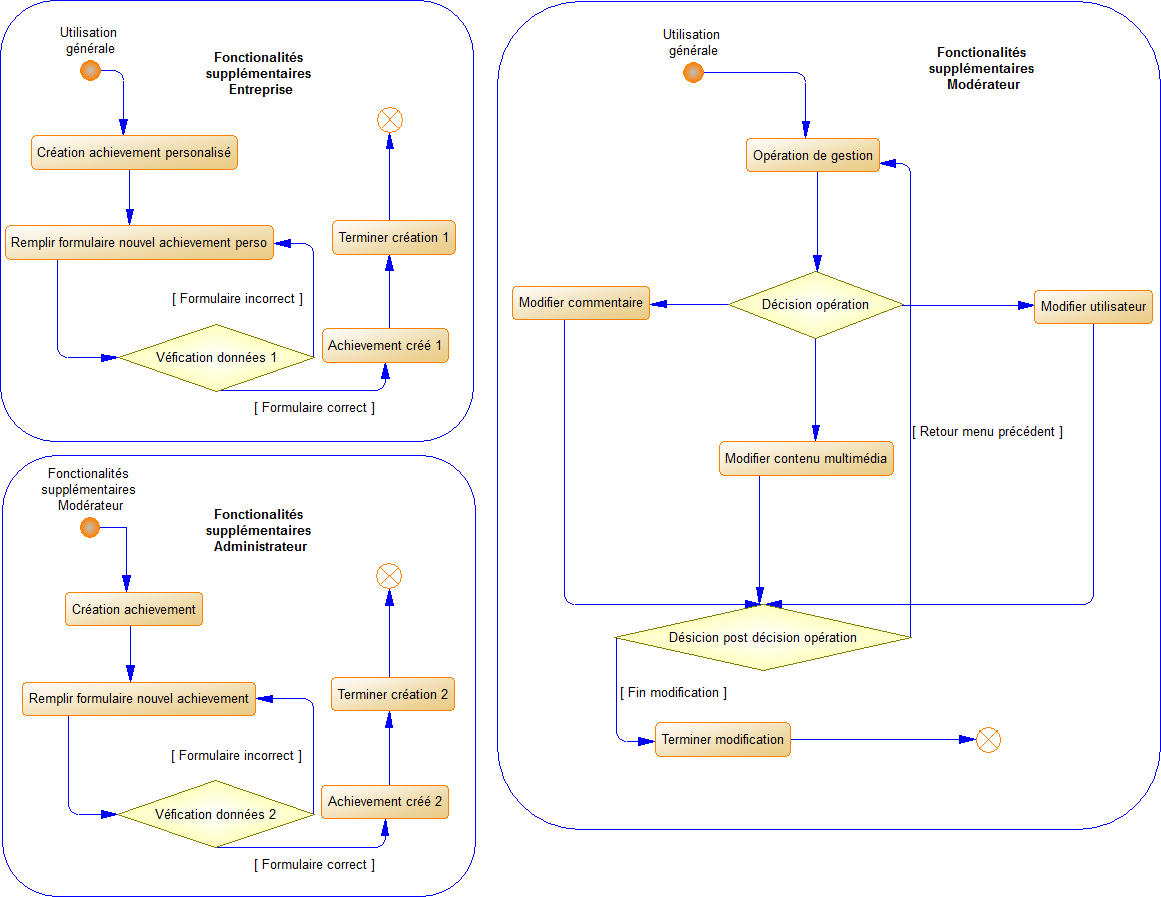
\includegraphics[width=17cm]{img/processus_principaux_1.png}
  \end{center}
\end{figure}

\vskip 3cm

\begin{figure}[H]
  \begin{center}
    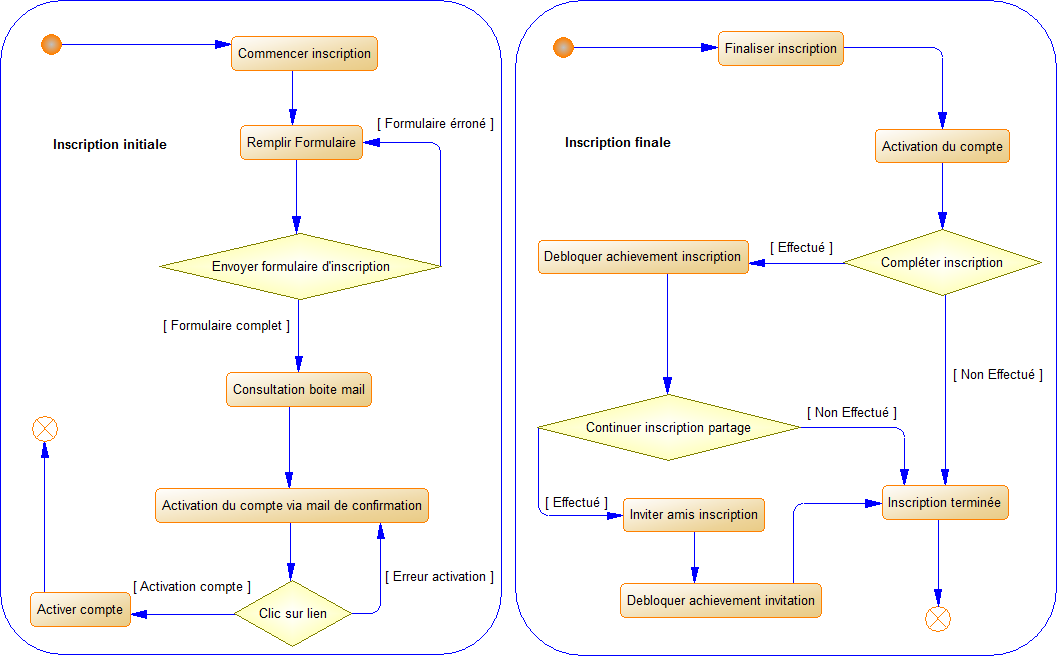
\includegraphics[width=17cm]{img/processus_detailles.png}
  \end{center}
\end{figure}

% --------------------------------------------------------------------- %%

\chapter{Vue Déploiement}
%% Vous présenterez ici la vue physique de votre application (Serveurs, liens réseau, protocoles, communication, et décrirez les éléments physiques en jeu lors des différents processus (présentés dans le chapitre précédent). Vous pourrez utiliser des diagrammes de déploiement UML. Vous préciserez aussi la partie gestion de la configuration qui permet de connaitre les contraintes de configuration de votre environnement cible. 

Le schéma présent sur la page suivante détaille le déploiement de l'application sur le serveur de développement, les différents services utilisés : bases de données, serveurs.

\newpage

\begin{figure}[H]
  \begin{center}
    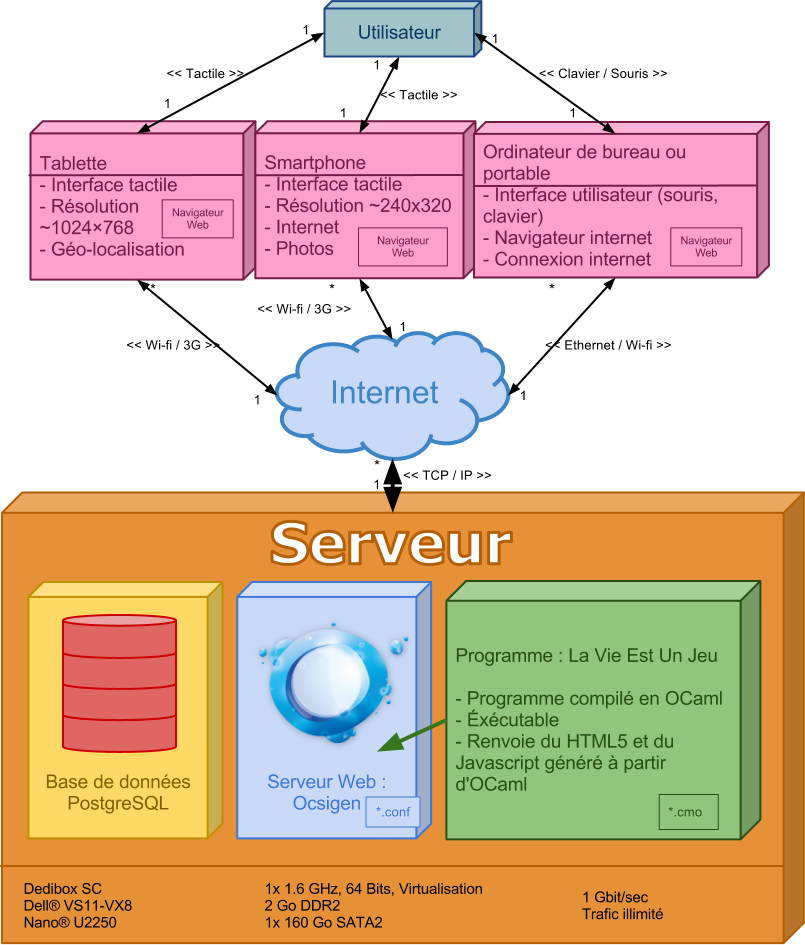
\includegraphics[width=17cm]{img/deploiement.png}
  \end{center}
\end{figure}


% --------------------------------------------------------------------- %%

\chapter{Implémentation}
\section{Vue globale}
%% Vous présenterez ici votre architecture logicielle à proprement parler, de façon plus détaillée, modèle en couche, N-Tiers, MVC, MVVM, MVP, … Vous préciserez les limites de chaque systèmes pour identifier les composants de chaque module (diagramme de package, diagramme de composants UML) 

TODO

\section{Couches applicatives}
%% Vous présenterez ici une vue plus détaillée avec des diagrammes objets, diagramme de classe par couche / composant 

TODO

% --------------------------------------------------------------------- %%

\chapter{Vue données}
%% Vous présenterez, si vous en avez, une vue conceptuelle de votre modèle de données. Les captures d’écran de bases déjà implémentées sont à proscrire. 

\begin{figure}[H]
  \begin{center}
    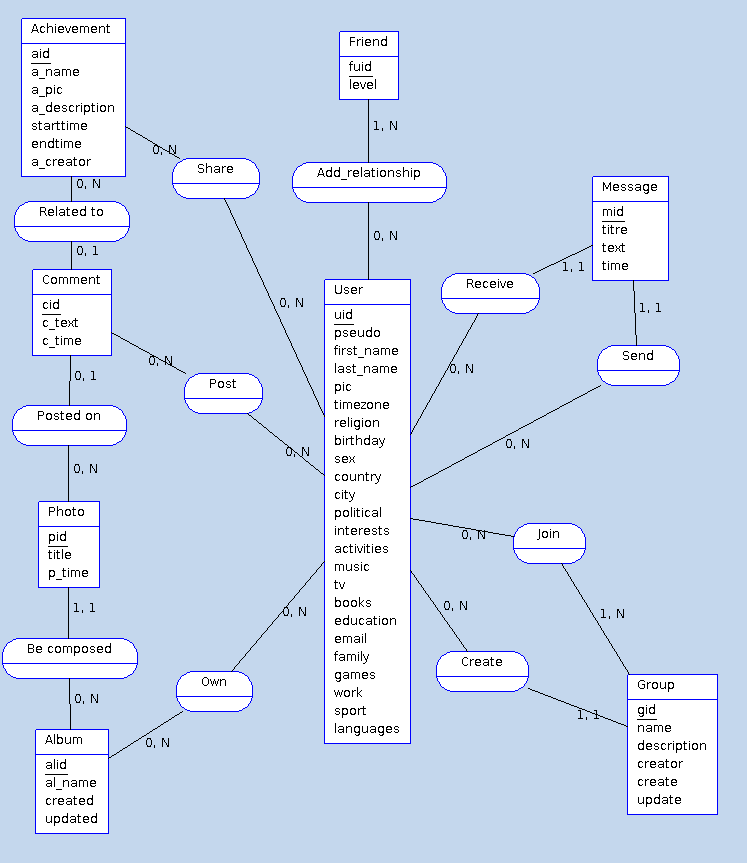
\includegraphics[width=17cm]{img/vue_donnees.png}
  \end{center}
\end{figure}

% --------------------------------------------------------------------- %%

\chapter{Taille et Performance}
%% Vous présenterez les ordres de grandeurs de la dimension de votre application dans cette section (nombre d’utilisateurs, de requête, taille du stockage de données, taille des requêtes, temps de réponse, localisation, …) 

Nous présenterons ici les différents chiffres relatifs à la dimension dans laquelle se positionnera notre application.\\
Pour la plupart des chiffres qui seront ici donnés, tout reste prévisionnel donc approximatif.\\

\begin{description}
  \item[Nombre d’utilisateurs :]
    Illimité, ou tout du moins la limite du nombre de personne utilisant internet, notre application s’adressant à tous et toute. Nous seront également probablement limités par les capacités en accueil de notre hébergeur.
  \item[Taille du stockage de données :]
    Nous aurons besoin d’un espace assez conséquent de stockage, chaque utilisateur ayant la possibilité de publier des photos et des vidéos, mais aussi de laisser des commentaires. Ainsi, plusieurs To ne seraient pas de trop.
  \item[Taille des requêtes :]
    Les requêtes sont variables.
  \item[Temps de réponse :]
    Du fait de la nature de notre application, les temps de réponse ne seront pas notre premier axe d’effort comme ce pourrait être le cas dans un jeu par exemple.
  \item[Localisation :]
    Nous avons pour ambition de proposer notre produit pour un maximum de plates-formes, ainsi, depuis n’importe quel terminal disposant d’un accès à internet, il sera possible d’accéder à notre application.
\end{description}

% --------------------------------------------------------------------- %%

\chapter{Qualité}
%% Une description de la façon dont l'architecture logicielle contribue à toutes les exigences (autres que fonctionnelles) du système: l'extensibilité, la fiabilité, la portabilité, et ainsi de suite. Si ces caractéristiques ont une importance particulière, pour les implications de sécurité, de sécurité ou de confidentialité, par exemple, ils devraient être clairement définis.

La plus grande force de la structure du service reste sa modularité. Ainsi, le projet se découpe en plusieurs binaires plus ou moins indépendants les uns des autres, ce qui offre différents avantages sous différents points de vue.\\
\\
D’abord, cette indépendance relative permet une disposition des ressources plus libre, ce qui est intéressant d’un point de vue pratique ou dans une optique d’optimisation. Ainsi, la base de donnée peut être installé sur une machine autre que celle du serveur web, ou encore du serveur réservé aux clients sur smartphones.\\
\\
Ensuite, cette organisation permet un usage de langages et de patterns plus ciblé et plus adapté aux fonctions des différents binaires. Cette dernière force également un certain niveau d’abstraction, qui en plus d'être un gage de stabilité du produit, permettra éventuellement d'étendre la portabilité du produit à l’avenir.\\
\\
Enfin, cette non centralisation des ressources est une mesure de sécurité efficace. En effet, il est intéressant de limiter les dangers éventuels d’une attaque ou d’une perte de données à un seul élément du projet, afin de limiter la casse et de protéger le reste.

%% --------------------------------------------------------------------- %%

\chapter{Conclusion}

TODO


\end{document}
